This chapter introduces baseline results and our results.

\section{Winoground}

\subsection{Compared To Humans}

\subsubsection{Baseline}

We show baseline results in \cref{tab:results_aggr_baseline}, which includes the following multimodal transformers: CLIP \cite{radford2021clip}, FLAVA \cite{singh2022flava}, LXMERT \cite{tan2020lxmert}, UniT \cite{hu2021unit}, UNITER \cite{chen2020uniter}, VILLA \cite{gan2020villa}, VinVL \cite{zhang2021vinvl}, ViLT \cite{kim2021vilt}, VisualBERT \cite{li2019visualbert} and ViLBERT \cite{lu2019vilbert}. They also evaluate several configurations of two types of RNN-based models: VSE++ \cite{faghri2018vse} and VSRN \cite{li2019vsrn}.

\begin{table}[ht]
\centering
\begin{tabular}{l|rrr|rrr}
\toprule
 &
  \multicolumn{3}{c|}{{Score}} &
  \multicolumn{3}{c}{{Accuracy}} \\
 Model                               & Text           & Image          & Group          & Text       & Image      & Group      \\
\midrule
 MTurk Human                         & \textbf{89.50} & \textbf{88.50} & \textbf{85.50} & \textbf{93.75} & \textbf{93.88} & \textbf{93.81} \\
 Random Chance                       & 25.00          & 25.00          & 16.67          & 50.00          & 50.00          & 50.00          \\
 \midrule
 VinVL                        & \textbf{37.75} & 17.75          & 14.50          & \textbf{62.75} & \textbf{57.75} & \textbf{60.25} \\
 UNITER$_{large}$             & \textbf{38.00} & 14.00          & 10.50          & \textbf{63.25} & \textbf{55.75} & \textbf{59.50} \\
 UNITER$_{base}$              & \textbf{32.25} & 13.25          & 10.00          & \textbf{60.62} & \textbf{55.50} & \textbf{58.06} \\
 ViLLA$_{large}$              & \textbf{37.00} & 13.25          & 11.00          & \textbf{62.62} & \textbf{55.25} & \textbf{58.94} \\
 ViLLA$_{base}$               & \textbf{30.00} & 12.00          & 8.00           & \textbf{59.62} & \textbf{55.00} & \textbf{57.31} \\
 VisualBERT$_{base}$          & 15.50          & 2.50           & 1.50           & \textbf{50.50} & 49.88          & \textbf{50.19} \\
 ViLT (ViT-B/32)              & \textbf{34.75} & 14.00          & 9.25           & \textbf{60.50} & \textbf{55.38} & \textbf{57.94} \\
 LXMERT                       & 19.25          & 7.00           & 4.00           & \textbf{52.12} & \textbf{51.88} & \textbf{52.00} \\
 ViLBERT$_{base}$             & 23.75          & 7.25           & 4.75           & \textbf{57.25} & \textbf{52.50} & \textbf{54.87} \\
 UniT$_{ITM Finetuned}$       & 19.50          & 6.25           & 4.00           & \textbf{50.25} & \textbf{50.75} & \textbf{50.50} \\
 FLAVA$_{ITM}$                & \textbf{32.25} & 20.50          & 14.25          & \textbf{62.75} & \textbf{59.13} & \textbf{60.94} \\
 FLAVA$_{Contrastive}$        & \textbf{25.25} & 13.50          & 9.00           & \textbf{59.25} & \textbf{55.12} & \textbf{57.19} \\
 CLIP (ViT-B/32)              & \textbf{30.75} & 10.50          & 8.00           & \textbf{60.38} & \textbf{53.25} & \textbf{56.81} \\
 VSE++$_{COCO}$ (ResNet)      & 22.75          & 8.00           & 4.00           & \textbf{51.38} & \textbf{50.88} & \textbf{51.12} \\
 VSE++$_{COCO}$ (VGG)         & 18.75          & 5.50           & 3.50           & \textbf{50.38} & 49.75          & \textbf{50.06} \\
 VSE++$_{Flickr30k}$ (ResNet) & 20.00          & 5.00           & 2.75           & \textbf{51.50} & \textbf{50.25} & \textbf{50.88} \\
 VSE++$_{Flickr30k}$ (VGG)    & 19.75          & 6.25           & 4.50           & \textbf{52.75} & \textbf{51.00} & \textbf{51.88} \\
 VSRN$_{COCO}$                & 17.50          & 7.00           & 3.75           & \textbf{50.38} & \textbf{51.12} & \textbf{50.75} \\
 VSRN$_{Flickr30k}$           & 20.00          & 5.00           & 3.50           & \textbf{53.25} & \textbf{51.75} & \textbf{52.50} \\
\bottomrule
\end{tabular}
\caption{Results on the Winoground dataset across the text, image and group score and accuracy metrics. Results above random chance in \textbf{bold}.}
\label{tab:results_aggr_baseline}
\end{table}

\subsubsection{Ours}

We show our results in \cref{tab:results_aggr_ours}, which includes various configurations of the following multimodal transformers: OFA \cite{wang2022unifying}, BLIP \cite{li2022blip}, CLIP \cite{radford2021clip}, FLAVA \cite{singh2022flava} and ViLT \cite{kim2021vilt}.

We test 4 different versions of ViLT. The first one is the pre-trained only version, without finetuning. Two others are finetuned for retrieval on COCO and Flickr30k. The last one is finetuned for visual reasoning on NLVR2. The best one is the one trained on NLVR2, which shows that finetuning on that task helps perform better on Winoground. Finetuning for retrieval is also helpful and improves the results of the pre-trained model. The score of the pre-trained model is lower than the baseline one.

For FLAVA and CLIP we manage to replicate baseline results. We also test 3 other CLIP models with different configurations and find that they all perform similar to the baseline configuration.

We test the 5 model sizes of OFA. Taking into account that this model gets state-of-the-art performance on many tasks, the performance is not very good. Even the biggest model is not better than the best baseline model. OFA is trained to generate "yes" or "no" when given an image and the text "Does the image describe <caption>?". This might explain why it does not perform that well on retrieval and Winoground.

We test many configurations of BLIP, which include different training sizes, scoring, vision transformer sizes and finetuning datasets. ITM score is better than ITC score in all the cases. Even the 14M pretrained only model is better than all the previously tested models. Finetuning for retrieval on COCO and Flickr30k improves the results even more, reaching nearly above random performance in text, image and group scores.

However, even the best model is still far from human performance in text, image and group scores. If we look at accuracy metrics, the gap is reduced, but the difference is still very big. Image score remains much lower than text score for all the models.

\begin{table}[ht]
\centering
\begin{tabular}{l|rrr|rrr}
\toprule
 &
  \multicolumn{3}{c|}{{Score}} &
  \multicolumn{3}{c}{{Accuracy}} \\
 Model                               & Text           & Image          & Group          & Text       & Image      & Group      \\
\midrule
 MTurk Human                         & \textbf{89.50} & \textbf{88.50} & \textbf{85.50} & \textbf{93.75} & \textbf{93.88} & \textbf{93.81} \\
 Random Chance                       & 25.00          & 25.00          & 16.67          & 50.00          & 50.00          & 50.00          \\
 \midrule
  ViLT (ViT-B/32)                     & \textbf{27.50} & 8.75           & 6.00           & \textbf{56.88} & \textbf{53.12} & \textbf{55.00} \\
 ViLT$_{COCO}$ (ViT-B/32)            & \textbf{32.75} & 13.50          & 11.25          & \textbf{61.88} & \textbf{56.00} & \textbf{58.94} \\
 ViLT$_{Flickr30k}$ (ViT-B/32)       & \textbf{35.00} & 11.50          & 9.75           & \textbf{61.62} & \textbf{54.50} & \textbf{58.06} \\
 ViLT$_{NLVR2}$ (ViT-B/32)           & \textbf{38.00} & 15.25          & 12.00          & \textbf{58.75} & \textbf{55.62} & \textbf{57.19} \\
 FLAVA$_{ITM}$                       & \textbf{32.25} & 20.50          & 14.25          & \textbf{62.75} & \textbf{59.13} & \textbf{60.94} \\
 FLAVA$_{ITC}$                       & \textbf{25.25} & 13.50          & 9.00           & \textbf{59.25} & \textbf{55.12} & \textbf{57.19} \\
 CLIP (ViT-B/32)                     & \textbf{30.75} & 10.25          & 8.25           & \textbf{60.38} & \textbf{53.12} & \textbf{56.75} \\
 CLIP (ViT-B/16)                     & 25.00          & 10.25          & 7.00           & \textbf{57.88} & \textbf{53.75} & \textbf{55.81} \\
 CLIP (ViT-L/14)                     & \textbf{28.50} & 11.00          & 8.00           & \textbf{60.38} & \textbf{54.62} & \textbf{57.50} \\
 CLIP (ViT-L/14-336)                 & \textbf{27.50} & 12.00          & 8.00           & \textbf{59.38} & \textbf{55.12} & \textbf{57.25} \\
 OFA$_{Tiny}$                        & 20.50          & 8.00           & 3.75           & \textbf{53.50} & \textbf{52.00} & \textbf{52.75} \\
 OFA$_{Base}$                        & \textbf{26.50} & 10.50          & 7.00           & \textbf{58.88} & \textbf{54.00} & \textbf{56.44} \\
 OFA$_{Medium}$                      & 22.75          & 9.00           & 5.50           & \textbf{54.25} & \textbf{52.75} & \textbf{53.50} \\
 OFA$_{Large}$                       & \textbf{26.00} & 8.75           & 5.75           & \textbf{58.38} & \textbf{52.88} & \textbf{55.62} \\
 OFA$_{Huge}$                        & \textbf{36.25} & 15.50          & 13.50          & \textbf{64.38} & \textbf{56.62} & \textbf{60.50} \\
 BLIP$_{ITM 14M}$ (ViT-B/16)         & \textbf{39.25} & 19.00          & 15.00          & \textbf{65.88} & \textbf{58.25} & \textbf{62.06} \\
 BLIP$_{ITC 14M}$ (ViT-B/16)         & \textbf{32.25} & 13.75          & 10.50          & \textbf{62.25} & \textbf{56.50} & \textbf{59.38} \\
 BLIP$_{ITM}$ (ViT-B/16)             & \textbf{40.50} & 20.50          & 16.50          & \textbf{66.25} & \textbf{59.00} & \textbf{62.62} \\
 BLIP$_{ITC}$ (ViT-B/16)             & \textbf{29.75} & 14.50          & 9.50           & \textbf{59.88} & \textbf{56.12} & \textbf{58.00} \\
 BLIP$_{ITM}$ (ViT-B/16) (CapFilt-L) & \textbf{37.50} & 18.50          & 14.00          & \textbf{65.00} & \textbf{59.13} & \textbf{62.06} \\
 BLIP$_{ITC}$ (ViT-B/16) (CapFilt-L) & \textbf{31.50} & 10.50          & 8.50           & \textbf{61.38} & \textbf{53.62} & \textbf{57.50} \\
 BLIP$_{ITM}$ (ViT-L/16)             & \textbf{42.50} & 18.25          & 15.50          & \textbf{66.88} & \textbf{57.25} & \textbf{62.06} \\
 BLIP$_{ITC}$ (ViT-L/16)             & \textbf{33.25} & 12.00          & 9.00           & \textbf{61.75} & \textbf{55.00} & \textbf{58.38} \\
 BLIP$_{ITM COCO}$ (ViT-B/16)        & \textbf{48.00} & 24.50          & \textbf{20.00} & \textbf{69.88} & \textbf{61.25} & \textbf{65.56} \\
 BLIP$_{ITC COCO}$ (ViT-B/16)        & \textbf{37.75} & 15.75          & 12.75          & \textbf{65.00} & \textbf{56.88} & \textbf{60.94} \\
 BLIP$_{ITM Flickr30k}$ (ViT-B/16)   & \textbf{46.25} & 24.25          & \textbf{21.25} & \textbf{69.25} & \textbf{60.62} & \textbf{64.94} \\
 BLIP$_{ITC Flickr30k}$ (ViT-B/16)   & \textbf{38.25} & 15.00          & 12.25          & \textbf{65.38} & \textbf{56.12} & \textbf{60.75} \\
 BLIP$_{ITM COCO}$ (ViT-L/16)        & \textbf{46.75} & 24.00          & \textbf{20.50} & \textbf{68.88} & \textbf{61.00} & \textbf{64.94} \\
 BLIP$_{ITC COCO}$ (ViT-L/16)        & \textbf{37.75} & 13.75          & 10.50          & \textbf{64.88} & \textbf{55.75} & \textbf{60.31} \\
 BLIP$_{ITM Flickr30k}$ (ViT-L/16)   & \textbf{45.00} & 24.75          & \textbf{20.50} & \textbf{68.62} & \textbf{60.50} & \textbf{64.56} \\
 BLIP$_{ITC Flickr30k}$ (ViT-L/16)   & \textbf{36.00} & 16.25          & 13.50          & \textbf{63.38} & \textbf{56.75} & \textbf{60.06} \\
\bottomrule
\end{tabular}
\caption{Results on the Winoground dataset across the text, image and group score and accuracy metrics. Results above random chance in \textbf{bold}.}
\label{tab:results_aggr_ours}
\end{table}

\subsection{Results By Linguistic Tag}

\subsubsection{Baseline}

See \cref{tab:results-by-ling-tag-baseline}

\begin{table}[ht]
    \centering
    \begin{adjustbox}{max width=\textwidth}
  \begin{tabular}{l|rrr|rrr|rrr|rrr|rrr}
    \toprule
     &
      \multicolumn{3}{c|}{Object} &
      \multicolumn{3}{c|}{Relation} &
      \multicolumn{3}{c|}{Both} &
      \multicolumn{3}{c|}{1 Main Pred} &
      \multicolumn{3}{c}{2 Main Preds}\\
    Model & Text & Image & Group & Text & Image & Group & Text & Image & Group & Text & Image & Group & Text & Image & Group \\\midrule
 MTurk Human                  & \textbf{92.20} & \textbf{90.78} & \textbf{88.65} & \textbf{89.27} & \textbf{90.56} & \textbf{86.70} & \textbf{76.92} & \textbf{57.69} & \textbf{57.69} & \textbf{87.33} & \textbf{85.62} & \textbf{82.53} & \textbf{95.37} & \textbf{96.30} & \textbf{93.52} \\
 VinVL                        & \textbf{36.88} & 17.73          & 14.18          & \textbf{37.77} & 17.60          & 14.16          & \textbf{42.31} & 19.23          & \textbf{19.23} & \textbf{39.38} & 21.23          & \textbf{17.47} & \textbf{33.33} & 8.33           & 6.48           \\
 UNITER$_{large}$             & \textbf{39.01} & 12.77          & 9.93           & \textbf{36.05} & 14.16          & 9.87           & \textbf{50.00} & 19.23          & \textbf{19.23} & \textbf{40.07} & 16.44          & 13.36          & \textbf{32.41} & 7.41           & 2.78           \\
 UNITER$_{base}$              & \textbf{34.04} & 11.35          & 9.22           & \textbf{30.04} & 14.16          & 10.30          & \textbf{42.31} & 15.38          & 11.54          & \textbf{35.27} & 14.73          & 11.99          & 24.07          & 9.26           & 4.63           \\
 ViLLA$_{large}$              & \textbf{36.88} & 14.89          & 11.35          & \textbf{37.34} & 12.88          & 11.16          & \textbf{34.62} & 7.69           & 7.69           & \textbf{39.73} & 17.12          & 14.38          & \textbf{29.63} & 2.78           & 1.85           \\
 ViLLA$_{base}$               & \textbf{33.33} & 15.60          & 9.93           & \textbf{27.04} & 9.01           & 6.01           & \textbf{38.46} & 19.23          & 15.38          & \textbf{33.22} & 14.04          & 10.27          & 21.30          & 6.48           & 1.85           \\
 VisualBERT$_{base}$          & 19.15          & 2.13           & 0.71           & 12.88          & 2.15           & 1.72           & 19.23          & 7.69           & 3.85           & 16.44          & 2.74           & 1.71           & 12.96          & 1.85           & 0.93           \\
 ViLT (ViT-B/32)              & \textbf{31.91} & 15.60          & 9.22           & \textbf{36.91} & 11.59          & 8.15           & \textbf{30.77} & \textbf{26.92} & \textbf{19.23} & \textbf{35.27} & 17.12          & 11.64          & \textbf{33.33} & 5.56           & 2.78           \\
 LXMERT                       & 22.70          & 9.22           & 6.38           & 17.60          & 5.58           & 2.58           & 15.38          & 7.69           & 3.85           & 19.18          & 8.56           & 5.14           & 19.44          & 2.78           & 0.93           \\
 ViLBERT$_{base}$             & \textbf{29.08} & 10.64          & 7.09           & 19.31          & 3.00           & 1.72           & \textbf{34.62} & \textbf{26.92} & \textbf{19.23} & 23.97          & 8.90           & 5.82           & 23.15          & 2.78           & 1.85           \\
 UniT$_{ITM finetuned}$       & 17.73          & 5.67           & 2.13           & 18.03          & 4.72           & 3.43           & \textbf{42.31} & 23.08          & \textbf{19.23} & 21.58          & 6.85           & 4.11           & 13.89          & 4.63           & 3.70           \\
  FLAVA$_{ITM}$                & \textbf{31.91} & 23.40 & 14.89 & \textbf{30.04} & 16.31 & 12.02 & \textbf{53.85} & \textbf{42.31} & \textbf{30.77} & \textbf{36.30} & 24.66 & \textbf{17.81} & 21.30          & 9.26 & 4.63 \\
 FLAVA$_{Contrastive}$        & 23.40          & 19.15 & 11.35 & 23.61          &  8.58 &  5.58 & \textbf{50.00} & \textbf{26.92} & \textbf{26.92} & \textbf{26.37} & 16.44 & 10.62          & 22.22          &  5.56 & 4.63 \\
 CLIP (ViT-B/32)              & \textbf{34.75} & 7.80           & 6.38           & 22.75          & 8.58           & 5.58           & \textbf{80.77} & \textbf{42.31} & \textbf{38.46} & \textbf{35.27} & 13.01          & 10.27          & 18.52          & 3.70           & 1.85           \\
 VSE++$_{COCO}$ (ResNet)      & 21.99          & 6.38           & 1.42           & 23.61          & 9.01           & 5.58           & 19.23          & 7.69           & 3.85           & 25.00          & 9.59           & 4.79           & 16.67          & 3.70           & 1.85           \\
 VSE++$_{COCO}$ (VGG)         & 17.73          & 2.13           & 2.13           & 18.45          & 7.30           & 3.86           & \textbf{26.92} & 7.69           & 7.69           & 18.49          & 4.79           & 2.74           & 19.44          & 7.41           & 5.56           \\
 VSE++$_{Flickr30k}$ (ResNet) & 20.57          & 6.38           & 3.55           & 18.88          & 4.29           & 2.15           & \textbf{26.92} & 3.85           & 3.85           & 21.58          & 6.51           & 3.42           & 15.74          & 0.93           & 0.93           \\
 VSE++$_{Flickr30k}$ (VGG)    & 17.73          & 4.96           & 2.84           & 19.74          & 6.87           & 5.15           & \textbf{30.77} & 7.69           & 7.69           & 20.55          & 6.16           & 4.79           & 17.59          & 6.48           & 3.70           \\
 VSRN$_{COCO}$                & 15.60          & 4.96           & 2.13           & 18.88          & 7.73           & 4.72           & 15.38          & 11.54          & 3.85           & 17.12          & 7.19           & 3.77           & 18.52          & 6.48           & 3.70           \\
 VSRN$_{Flickr30k}$           & 16.31          & 4.96           & 2.13           & 21.03          & 4.29           & 3.86           & \textbf{30.77} & 11.54          & 7.69           & 20.89          & 5.82           & 3.77           & 17.59          & 2.78           & 2.78           \\
          \bottomrule
  \end{tabular}
  \end{adjustbox}
  \caption{The results by linguistic tag. Results above chance are in \textbf{bold}.}
    \label{tab:results-by-ling-tag-baseline}
\end{table}

\subsubsection{Ours}

See \cref{tab:results-by-ling-tag-ours}

\begin{table}[ht]
    \centering
    \begin{adjustbox}{max width=\textwidth}
  \begin{tabular}{l|rrr|rrr|rrr|rrr|rrr}
    \toprule
     &
      \multicolumn{3}{c|}{Object} &
      \multicolumn{3}{c|}{Relation} &
      \multicolumn{3}{c|}{Both} &
      \multicolumn{3}{c|}{1 Main Pred} &
      \multicolumn{3}{c}{2 Main Preds}\\
    Model & Text & Image & Group & Text & Image & Group & Text & Image & Group & Text & Image & Group & Text & Image & Group \\\midrule
 MTurk Human                  & \textbf{92.20} & \textbf{90.78} & \textbf{88.65} & \textbf{89.27} & \textbf{90.56} & \textbf{86.70} & \textbf{76.92} & \textbf{57.69} & \textbf{57.69} & \textbf{87.33} & \textbf{85.62} & \textbf{82.53} & \textbf{95.37} & \textbf{96.30} & \textbf{93.52} \\
  ViLT (ViT-B/32)                     & \textbf{29.08} & 10.64          & 4.96           & \textbf{26.18} & 7.73           & 6.44           & \textbf{30.77} & 7.69           & 7.69           & \textbf{30.14} & 10.62          & 7.53           & 20.37          & 3.70           & 1.85           \\
 ViLT$_{COCO}$ (ViT-B/32)            & \textbf{33.33} & 15.60          & 12.77          & \textbf{30.90} & 10.73          & 9.01           & \textbf{46.15} & \textbf{26.92} & \textbf{23.08} & \textbf{36.64} & 15.75          & 14.04          & 22.22          & 7.41           & 3.70           \\
 ViLT$_{Flickr30k}$ (ViT-B/32)       & \textbf{32.62} & 14.89          & 11.35          & \textbf{35.62} & 8.15           & 7.73           & \textbf{42.31} & 23.08          & \textbf{19.23} & \textbf{36.99} & 14.38          & 11.99          & \textbf{29.63} & 3.70           & 3.70           \\
 ViLT$_{NLVR2}$ (ViT-B/32)           & \textbf{39.01} & 16.31          & 14.18          & \textbf{36.48} & 14.59          & 10.30          & \textbf{46.15} & 15.38          & 15.38          & \textbf{39.73} & 18.15          & 15.07          & \textbf{33.33} & 7.41           & 3.70           \\
 FLAVA$_{ITM}$                       & \textbf{31.91} & 23.40          & 14.89          & \textbf{30.04} & 16.31          & 12.02          & \textbf{53.85} & \textbf{42.31} & \textbf{30.77} & \textbf{36.30} & 24.66          & \textbf{17.81} & 21.30          & 9.26           & 4.63           \\
 FLAVA$_{ITC}$                       & 23.40          & 19.15          & 11.35          & 23.61          & 8.58           & 5.58           & \textbf{50.00} & \textbf{26.92} & \textbf{26.92} & \textbf{26.37} & 16.44          & 10.62          & 22.22          & 5.56           & 4.63           \\
 CLIP (ViT-B/32)                     & \textbf{35.46} & 7.80           & 6.38           & 22.32          & 7.73           & 5.58           & \textbf{80.77} & \textbf{46.15} & \textbf{42.31} & \textbf{35.62} & 13.01          & 10.62          & 17.59          & 2.78           & 1.85           \\
 CLIP (ViT-B/16)                     & \textbf{27.66} & 10.64          & 5.67           & 19.31          & 6.44           & 4.29           & \textbf{61.54} & \textbf{42.31} & \textbf{38.46} & \textbf{30.14} & 11.99          & 8.90           & 11.11          & 5.56           & 1.85           \\
 CLIP (ViT-L/14)                     & \textbf{27.66} & 8.51           & 5.67           & \textbf{25.75} & 9.87           & 6.44           & \textbf{57.69} & \textbf{34.62} & \textbf{34.62} & \textbf{30.14} & 13.01          & 9.93           & 24.07          & 5.56           & 2.78           \\
 CLIP (ViT-L/14-336)                 & \textbf{32.62} & 12.77          & 9.22           & 21.03          & 8.15           & 4.29           & \textbf{57.69} & \textbf{42.31} & \textbf{34.62} & \textbf{30.48} & 14.04          & 10.62          & 19.44          & 6.48           & 0.93           \\
 OFA$_{Tiny}$                        & 22.70          & 6.38           & 2.13           & 17.17          & 6.87           & 3.43           & \textbf{38.46} & \textbf{26.92} & 15.38          & 23.97          & 8.22           & 4.45           & 11.11          & 7.41           & 1.85           \\
 OFA$_{Base}$                        & \textbf{25.53} & 14.18          & 7.09           & 24.46          & 6.87           & 5.15           & \textbf{50.00} & 23.08          & \textbf{23.08} & \textbf{28.77} & 12.67          & 8.56           & 20.37          & 4.63           & 2.78           \\
 OFA$_{Medium}$                      & 19.86          & 7.80           & 4.26           & 22.32          & 7.73           & 4.72           & \textbf{42.31} & \textbf{26.92} & \textbf{19.23} & 24.32          & 10.96          & 6.85           & 18.52          & 3.70           & 1.85           \\
 OFA$_{Large}$                       & \textbf{26.24} & 10.64          & 5.67           & 24.03          & 5.15           & 3.86           & \textbf{42.31} & \textbf{30.77} & \textbf{23.08} & \textbf{29.45} & 10.96          & 7.53           & 16.67          & 2.78           & 0.93           \\
 OFA$_{Huge}$                        & \textbf{40.43} & 18.44          & 15.60          & \textbf{30.90} & 11.59          & 9.87           & \textbf{61.54} & \textbf{34.62} & \textbf{34.62} & \textbf{39.73} & 19.18          & \textbf{16.78} & \textbf{26.85} & 5.56           & 4.63           \\
 BLIP$_{ITM 14M}$ (ViT-B/16)         & \textbf{41.84} & 23.40          & \textbf{17.73} & \textbf{36.05} & 14.59          & 11.59          & \textbf{53.85} & \textbf{34.62} & \textbf{30.77} & \textbf{43.84} & 23.63          & \textbf{18.49} & \textbf{26.85} & 6.48           & 5.56           \\
 BLIP$_{ITC 14M}$ (ViT-B/16)         & \textbf{34.04} & 13.48          & 9.93           & \textbf{28.33} & 12.02          & 9.44           & \textbf{57.69} & \textbf{30.77} & \textbf{23.08} & \textbf{37.67} & 16.44          & 13.01          & 17.59          & 6.48           & 3.70           \\
 BLIP$_{ITM}$ (ViT-B/16)             & \textbf{46.10} & 22.70          & \textbf{17.73} & \textbf{35.62} & 17.60          & 14.16          & \textbf{53.85} & \textbf{34.62} & \textbf{30.77} & \textbf{45.89} & \textbf{25.34} & \textbf{20.55} & \textbf{25.93} & 7.41           & 5.56           \\
 BLIP$_{ITC}$ (ViT-B/16)             & \textbf{34.75} & 14.18          & 9.22           & \textbf{25.32} & 13.73          & 8.58           & \textbf{42.31} & 23.08          & \textbf{19.23} & \textbf{33.56} & 16.10          & 10.62          & 19.44          & 10.19          & 6.48           \\
 BLIP$_{ITM}$ (ViT-B/16) (CapFilt-L) & \textbf{39.01} & 19.86          & 12.77          & \textbf{34.76} & 15.88          & 12.45          & \textbf{53.85} & \textbf{34.62} & \textbf{34.62} & \textbf{41.10} & 22.60          & \textbf{17.12} & \textbf{27.78} & 7.41           & 5.56           \\
 BLIP$_{ITC}$ (ViT-B/16) (CapFilt-L) & \textbf{36.88} & 12.77          & 9.22           & \textbf{26.18} & 8.58           & 7.30           & \textbf{50.00} & 15.38          & 15.38          & \textbf{35.96} & 13.36          & 10.96          & 19.44          & 2.78           & 1.85           \\
 BLIP$_{ITM}$ (ViT-L/16)             & \textbf{41.84} & 19.86          & \textbf{17.02} & \textbf{40.77} & 16.31          & 13.73          & \textbf{61.54} & \textbf{26.92} & \textbf{23.08} & \textbf{45.55} & 23.29          & \textbf{20.21} & \textbf{34.26} & 4.63           & 2.78           \\
 BLIP$_{ITC}$ (ViT-L/16)             & \textbf{34.04} & 14.18          & 11.35          & \textbf{30.90} & 9.01           & 6.01           & \textbf{50.00} & \textbf{26.92} & \textbf{23.08} & \textbf{36.99} & 14.04          & 10.96          & 23.15          & 6.48           & 3.70           \\
 BLIP$_{ITM COCO}$ (ViT-B/16)        & \textbf{42.55} & \textbf{26.95} & \textbf{19.15} & \textbf{49.79} & 21.89          & \textbf{19.31} & \textbf{61.54} & \textbf{34.62} & \textbf{30.77} & \textbf{48.97} & \textbf{29.79} & \textbf{24.66} & \textbf{45.37} & 10.19          & 7.41           \\
 BLIP$_{ITC COCO}$ (ViT-B/16)        & \textbf{36.88} & 19.15          & 14.18          & \textbf{36.05} & 11.59          & 10.30          & \textbf{57.69} & \textbf{34.62} & \textbf{26.92} & \textbf{41.78} & 18.84          & 15.07          & \textbf{26.85} & 7.41           & 6.48           \\
 BLIP$_{ITM Flickr30k}$ (ViT-B/16)   & \textbf{49.65} & \textbf{28.37} & \textbf{22.70} & \textbf{42.49} & 19.74          & \textbf{18.45} & \textbf{61.54} & \textbf{42.31} & \textbf{38.46} & \textbf{51.03} & \textbf{28.42} & \textbf{26.03} & \textbf{33.33} & 12.96          & 8.33           \\
 BLIP$_{ITC Flickr30k}$ (ViT-B/16)   & \textbf{36.88} & 17.02          & 10.64          & \textbf{36.48} & 12.02          & 11.16          & \textbf{61.54} & \textbf{30.77} & \textbf{30.77} & \textbf{40.75} & 17.12          & 13.70          & \textbf{31.48} & 9.26           & 8.33           \\
 BLIP$_{ITM COCO}$ (ViT-L/16)        & \textbf{48.94} & \textbf{25.53} & \textbf{20.57} & \textbf{44.64} & 22.32          & \textbf{20.60} & \textbf{53.85} & \textbf{30.77} & \textbf{19.23} & \textbf{51.03} & \textbf{28.42} & \textbf{23.97} & \textbf{35.19} & 12.04          & 11.11          \\
 BLIP$_{ITC COCO}$ (ViT-L/16)        & \textbf{36.88} & 14.18          & 11.35          & \textbf{36.05} & 11.16          & 7.30           & \textbf{57.69} & \textbf{34.62} & \textbf{34.62} & \textbf{41.10} & 16.44          & 13.36          & \textbf{28.70} & 6.48           & 2.78           \\
 BLIP$_{ITM Flickr30k}$ (ViT-L/16)   & \textbf{46.10} & 22.70          & 16.31          & \textbf{42.06} & 24.89          & \textbf{21.46} & \textbf{65.38} & \textbf{34.62} & \textbf{34.62} & \textbf{50.34} & \textbf{29.11} & \textbf{24.66} & \textbf{30.56} & 12.96          & 9.26           \\
 BLIP$_{ITC Flickr30k}$ (ViT-L/16)   & \textbf{39.01} & 19.86          & 15.60          & \textbf{30.47} & 11.59          & 9.44           & \textbf{69.23} & \textbf{38.46} & \textbf{38.46} & \textbf{39.38} & 20.55          & \textbf{17.12} & \textbf{26.85} & 4.63           & 3.70           \\
          \bottomrule
  \end{tabular}
  \end{adjustbox}
  \caption{The results by linguistic tag. Results above chance are in \textbf{bold}.}
    \label{tab:results-by-ling-tag-ours}
\end{table}

\subsection{Results By Visual Tag}

\subsubsection{Baseline}

See \cref{tab:results-by-visual-tag-baseline}

\begin{table}[ht]
    \centering
   \begin{adjustbox}{max width=\textwidth}
  \begin{tabular}{l|rrr|rrr|rrr}
    \toprule
     &
      \multicolumn{3}{c|}{Symbolic} &
      \multicolumn{3}{c|}{Pragmatics} &
      \multicolumn{3}{c}{Same Image Series} \\
    Model & Text & Image & Group & Text & Image & Group & Text & Image & Group \\\midrule
 MTurk Human                  & \textbf{96.43} & \textbf{92.86} & \textbf{92.86} & \textbf{58.82} & \textbf{41.18} & \textbf{41.18} & \textbf{95.65} & \textbf{91.30} & \textbf{91.30} \\
 VinVL                        & 25.00          & 17.86          & 14.29          & \textbf{29.41} & 5.88           & 5.88           & \textbf{34.78} & 17.39          & 13.04          \\
 UNITER$_{large}$             & \textbf{39.29} & \textbf{28.57} & \textbf{17.86} & \textbf{35.29} & 0.00           & 0.00           & 4.35           & 8.70           & 0.00           \\
 UNITER$_{base}$              & \textbf{46.43} & 14.29          & 14.29          & \textbf{29.41} & 17.65          & 11.76          & 8.70           & 8.70           & 0.00           \\
 ViLLA$_{large}$              & \textbf{39.29} & 14.29          & 10.71          & 17.65          & 0.00           & 0.00           & 17.39          & 4.35           & 0.00           \\
 ViLLA$_{base}$               & \textbf{42.86} & 17.86          & 14.29          & \textbf{29.41} & 5.88           & 5.88           & 13.04          & 8.70           & 4.35           \\
 VisualBERT$_{base}$          & \textbf{28.57} & 0.00           & 0.00           & 5.88           & 0.00           & 0.00           & 13.04          & 0.00           & 0.00           \\
 ViLT (ViT-B/32)              & \textbf{28.57} & 17.86          & 10.71          & \textbf{35.29} & 0.00           & 0.00           & \textbf{26.09} & 0.00           & 0.00           \\
 LXMERT                       & \textbf{28.57} & 3.57           & 3.57           & 17.65          & 5.88           & 0.00           & 8.70           & 4.35           & 0.00           \\
 ViLBERT$_{base}$             & \textbf{28.57} & 10.71          & 7.14           & \textbf{29.41} & 5.88           & 5.88           & 13.04          & 0.00           & 0.00           \\
 UniT$_{ITM finetuned}$       & 14.29          & 10.71          & 7.14           & 17.65          & 5.88           & 5.88           & 21.74          & 4.35           & 4.35           \\
 FLAVA$_{ITM}$                & 25.00          & \textbf{28.57} & \textbf{17.86} & 17.65          & \textbf{29.41} & 11.76 & 17.39          &  8.70 &  0.00 \\
 FLAVA$_{Contrastive}$        & 17.86          & 10.71          & 10.71          & 11.76          & 23.53          & 5.88           & 17.39          & 4.35           &  4.35 \\
 CLIP (ViT-B/32)              & \textbf{39.29} & 3.57           & 3.57           & \textbf{35.29} & 5.88           & 5.88           & 8.70           & 0.00           & 0.00           \\
 VSE++$_{COCO}$ (ResNet)      & \textbf{32.14} & 10.71          & 10.71          & 23.53          & 11.76          & 0.00           & 13.04          & 4.35           & 4.35           \\
 VSE++$_{COCO}$ (VGG)         & 17.86          & 14.29          & 7.14           & 17.65          & 0.00           & 0.00           & 13.04          & 4.35           & 4.35           \\
 VSE++$_{Flickr30k}$ (ResNet) & 21.43          & 3.57           & 0.00           & 23.53          & 0.00           & 0.00           & 17.39          & 4.35           & 0.00           \\
 VSE++$_{Flickr30k}$ (VGG)    & \textbf{28.57} & 10.71          & 10.71          & 11.76          & 0.00           & 0.00           & 13.04          & 4.35           & 0.00           \\
 VSRN$_{COCO}$                & 7.14           & 3.57           & 0.00           & 11.76          & 0.00           & 0.00           & 13.04          & 0.00           & 0.00           \\
 VSRN$_{Flickr30k}$           & 21.43          & 3.57           & 3.57           & \textbf{35.29} & 11.76          & 5.88           & 8.70           & 4.35           & 4.35           \\
    \bottomrule
  \end{tabular}
  \end{adjustbox}
  \caption{The results by visual tag. Results above chance are in \textbf{bold}.}
    \label{tab:results-by-visual-tag-baseline}
\end{table}

\subsubsection{Ours}

See \cref{tab:results-by-visual-tag-ours}

\begin{table}[ht]
    \centering
   \begin{adjustbox}{max width=\textwidth}
  \begin{tabular}{l|rrr|rrr|rrr}
    \toprule
     &
      \multicolumn{3}{c|}{Symbolic} &
      \multicolumn{3}{c|}{Pragmatics} &
      \multicolumn{3}{c}{Same Image Series} \\
    Model & Text & Image & Group & Text & Image & Group & Text & Image & Group \\\midrule
 MTurk Human                  & \textbf{96.43} & \textbf{92.86} & \textbf{92.86} & \textbf{58.82} & \textbf{41.18} & \textbf{41.18} & \textbf{95.65} & \textbf{91.30} & \textbf{91.30} \\
ViLT (ViT-B/32)                     & 21.43          & 7.14           & 3.57           & 17.65          & 5.88           & 5.88           & 17.39          & 8.70           & 4.35           \\
 ViLT$_{COCO}$ (ViT-B/32)            & 21.43          & 10.71          & 10.71          & \textbf{29.41} & 17.65          & 5.88           & 21.74          & 8.70           & 4.35           \\
 ViLT$_{Flickr30k}$ (ViT-B/32)       & \textbf{28.57} & 7.14           & 7.14           & 23.53          & 0.00           & 0.00           & \textbf{26.09} & 4.35           & 4.35           \\
 ViLT$_{NLVR2}$ (ViT-B/32)           & \textbf{42.86} & 10.71          & 10.71          & \textbf{41.18} & 0.00           & 0.00           & 17.39          & 13.04          & 4.35           \\
 FLAVA$_{ITM}$                       & 25.00          & \textbf{28.57} & \textbf{17.86} & 17.65          & \textbf{29.41} & 11.76          & 17.39          & 8.70           & 0.00           \\
 FLAVA$_{ITC}$                       & 17.86          & 10.71          & 10.71          & 11.76          & 23.53          & 5.88           & 17.39          & 4.35           & 4.35           \\
 CLIP (ViT-B/32)                     & \textbf{35.71} & 3.57           & 3.57           & \textbf{35.29} & 5.88           & 5.88           & 13.04          & 0.00           & 0.00           \\
 CLIP (ViT-B/16)                     & 21.43          & 3.57           & 3.57           & \textbf{29.41} & 11.76          & 11.76          & 4.35           & 4.35           & 0.00           \\
 CLIP (ViT-L/14)                     & \textbf{28.57} & 10.71          & 3.57           & 23.53          & 17.65          & 11.76          & 13.04          & 8.70           & 4.35           \\
 CLIP (ViT-L/14-336)                 & \textbf{28.57} & 14.29          & 7.14           & 17.65          & 17.65          & 5.88           & 13.04          & 4.35           & 0.00           \\
 OFA$_{Tiny}$                        & 21.43          & 7.14           & 7.14           & 11.76          & 17.65          & 0.00           & 21.74          & 8.70           & 0.00           \\
 OFA$_{Base}$                        & \textbf{28.57} & 10.71          & 10.71          & 23.53          & 5.88           & 5.88           & 21.74          & 13.04          & 4.35           \\
 OFA$_{Medium}$                      & \textbf{28.57} & 10.71          & 7.14           & 17.65          & 5.88           & 5.88           & 13.04          & 8.70           & 4.35           \\
 OFA$_{Large}$                       & \textbf{28.57} & 14.29          & 10.71          & \textbf{29.41} & 0.00           & 0.00           & 13.04          & 0.00           & 0.00           \\
 OFA$_{Huge}$                        & \textbf{39.29} & 14.29          & 14.29          & 11.76          & 11.76          & 5.88           & 17.39          & 4.35           & 4.35           \\
 BLIP$_{ITM 14M}$ (ViT-B/16)         & \textbf{46.43} & 17.86          & \textbf{17.86} & \textbf{35.29} & 11.76          & 11.76          & 17.39          & 4.35           & 0.00           \\
 BLIP$_{ITC 14M}$ (ViT-B/16)         & \textbf{32.14} & 14.29          & 10.71          & \textbf{29.41} & 0.00           & 0.00           & 13.04          & 0.00           & 0.00           \\
 BLIP$_{ITM}$ (ViT-B/16)             & \textbf{50.00} & 17.86          & \textbf{17.86} & \textbf{29.41} & 5.88           & 5.88           & 13.04          & 4.35           & 0.00           \\
 BLIP$_{ITC}$ (ViT-B/16)             & \textbf{39.29} & 10.71          & 7.14           & 5.88           & 11.76          & 0.00           & 4.35           & 8.70           & 0.00           \\
 BLIP$_{ITM}$ (ViT-B/16) (CapFilt-L) & \textbf{42.86} & 17.86          & 14.29          & 23.53          & 17.65          & \textbf{17.65} & 17.39          & 4.35           & 0.00           \\
 BLIP$_{ITC}$ (ViT-B/16) (CapFilt-L) & \textbf{42.86} & 0.00           & 0.00           & 17.65          & 0.00           & 0.00           & 4.35           & 0.00           & 0.00           \\
 BLIP$_{ITM}$ (ViT-L/16)             & \textbf{53.57} & 25.00          & \textbf{25.00} & \textbf{29.41} & 5.88           & 0.00           & \textbf{26.09} & 4.35           & 0.00           \\
 BLIP$_{ITC}$ (ViT-L/16)             & \textbf{39.29} & 17.86          & 14.29          & \textbf{41.18} & 11.76          & 11.76          & 8.70           & 4.35           & 4.35           \\
 BLIP$_{ITM COCO}$ (ViT-B/16)        & \textbf{53.57} & 17.86          & \textbf{17.86} & \textbf{58.82} & 17.65          & \textbf{17.65} & \textbf{39.13} & 8.70           & 0.00           \\
 BLIP$_{ITC COCO}$ (ViT-B/16)        & 25.00          & 10.71          & 7.14           & \textbf{35.29} & 5.88           & 5.88           & 17.39          & 8.70           & 4.35           \\
 BLIP$_{ITM Flickr30k}$ (ViT-B/16)   & \textbf{53.57} & 21.43          & \textbf{21.43} & \textbf{35.29} & 11.76          & 11.76          & \textbf{26.09} & 4.35           & 4.35           \\
 BLIP$_{ITC Flickr30k}$ (ViT-B/16)   & \textbf{35.71} & 10.71          & 10.71          & 23.53          & 17.65          & 11.76          & 17.39          & 4.35           & 0.00           \\
 BLIP$_{ITM COCO}$ (ViT-L/16)        & \textbf{39.29} & \textbf{35.71} & \textbf{25.00} & \textbf{58.82} & 23.53          & \textbf{17.65} & \textbf{26.09} & 4.35           & 0.00           \\
 BLIP$_{ITC COCO}$ (ViT-L/16)        & \textbf{46.43} & 14.29          & 14.29          & 17.65          & 5.88           & 5.88           & 13.04          & 0.00           & 0.00           \\
 BLIP$_{ITM Flickr30k}$ (ViT-L/16)   & \textbf{39.29} & \textbf{28.57} & \textbf{25.00} & \textbf{47.06} & 11.76          & 5.88           & \textbf{30.43} & 8.70           & 4.35           \\
 BLIP$_{ITC Flickr30k}$ (ViT-L/16)   & \textbf{39.29} & 14.29          & 14.29          & \textbf{47.06} & 5.88           & 5.88           & 21.74          & 13.04          & 13.04          \\
\bottomrule
\end{tabular}
  \end{adjustbox}
  \caption{The results by visual tag. Results above chance are in \textbf{bold}.}
    \label{tab:results-by-visual-tag-ours}
\end{table}

\section{Visual Spatial Reasoning}

\subsection{Compared To Humans}

\subsubsection{Baseline}

See \cref{tab:vsr_results_base}. The gap between dev and tests becomes much greater on zero-shot split likely due to the smaller size of both dev and test sets.

\begin{table}[ht]
\centering
%\setlength{\tabcolsep}{2.8pt}
\small
\begin{tabular}{lcccccc}
\toprule
& \multicolumn{2}{c}{random split} &  & \multicolumn{2}{c}{zero-shot split} \\
\cmidrule(l){2-3} 	\cmidrule(l){4-6}
model$\downarrow$ & dev & test & & dev & test  \\
\midrule
human & \multicolumn{5}{c}{95.4}   \\
\midrule
VisualBERT & 59.2$_{\pm0.9}$ & 57.4$_{\pm0.9}$ & & 57.4$_{\pm2.2}$  & 54.0$_{\pm1.3}$  \\ 
LXMERT & \textbf{73.8}$_{\pm1.2}$  & \textbf{72.5}$_{\pm1.4}$ & & \textbf{69.2}$_{\pm1.0}$  & \textbf{63.2}$_{\pm1.7}$  \\ 
ViLT & 71.9$_{\pm1.3}$  & 71.0$_{\pm0.7}$  & & 66.7$_{\pm1.7}$  & 62.4$_{\pm1.5}$ \\ 
\bottomrule
\end{tabular}
\caption{Model performance on VSR. Results of both random and zero-shot splits, both validation and tests are listed.}
\label{tab:vsr_results_base}
\end{table}

\subsubsection{Ours}

\subsection{Results By Relation}

\subsubsection{Baseline}

See \cref{fig:performance_by_rel_base}

\begin{figure*}
    \centering
\begin{subfigure}[b]{\linewidth}
    \centering
    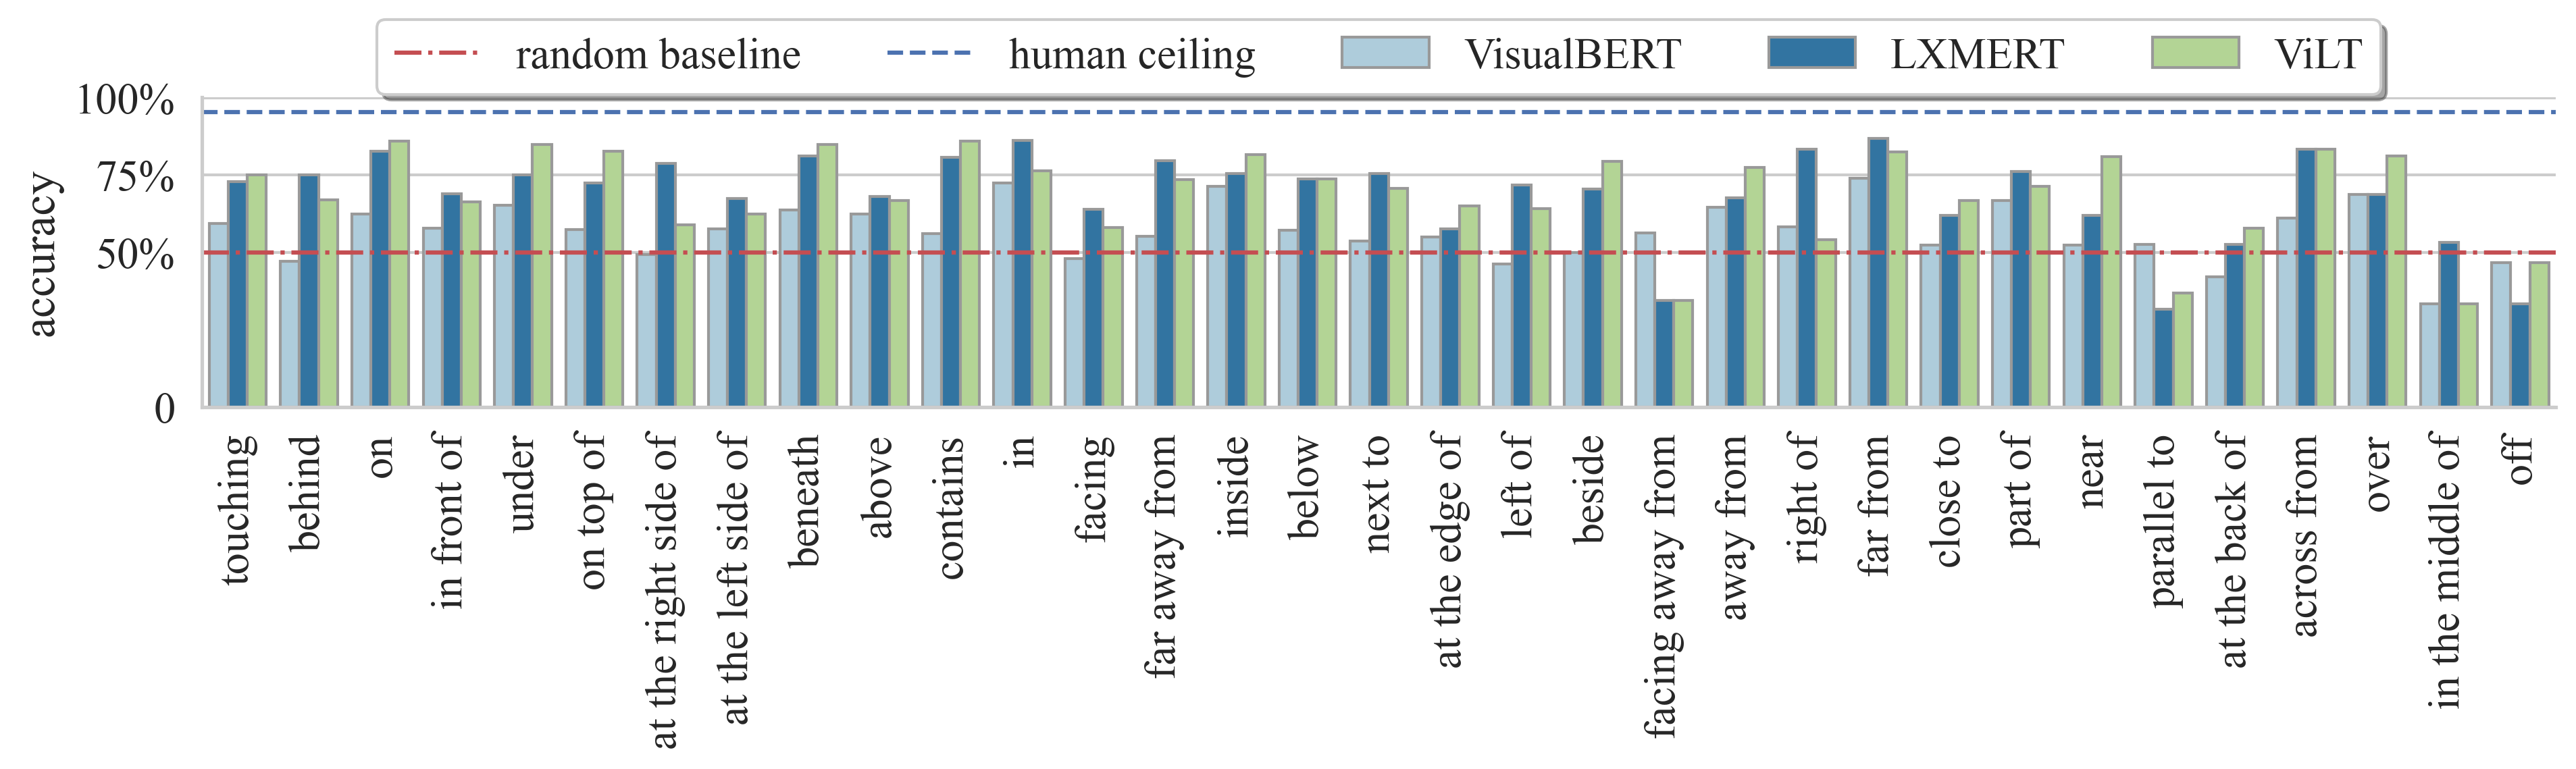
\includegraphics[width=\linewidth]{images/visual-spatial-reasoning/performance_by_relation_random_split_v2.png}
    \vspace{-1cm}
    \caption{random split}
\end{subfigure}
\begin{subfigure}[b]{\linewidth}
    \centering
    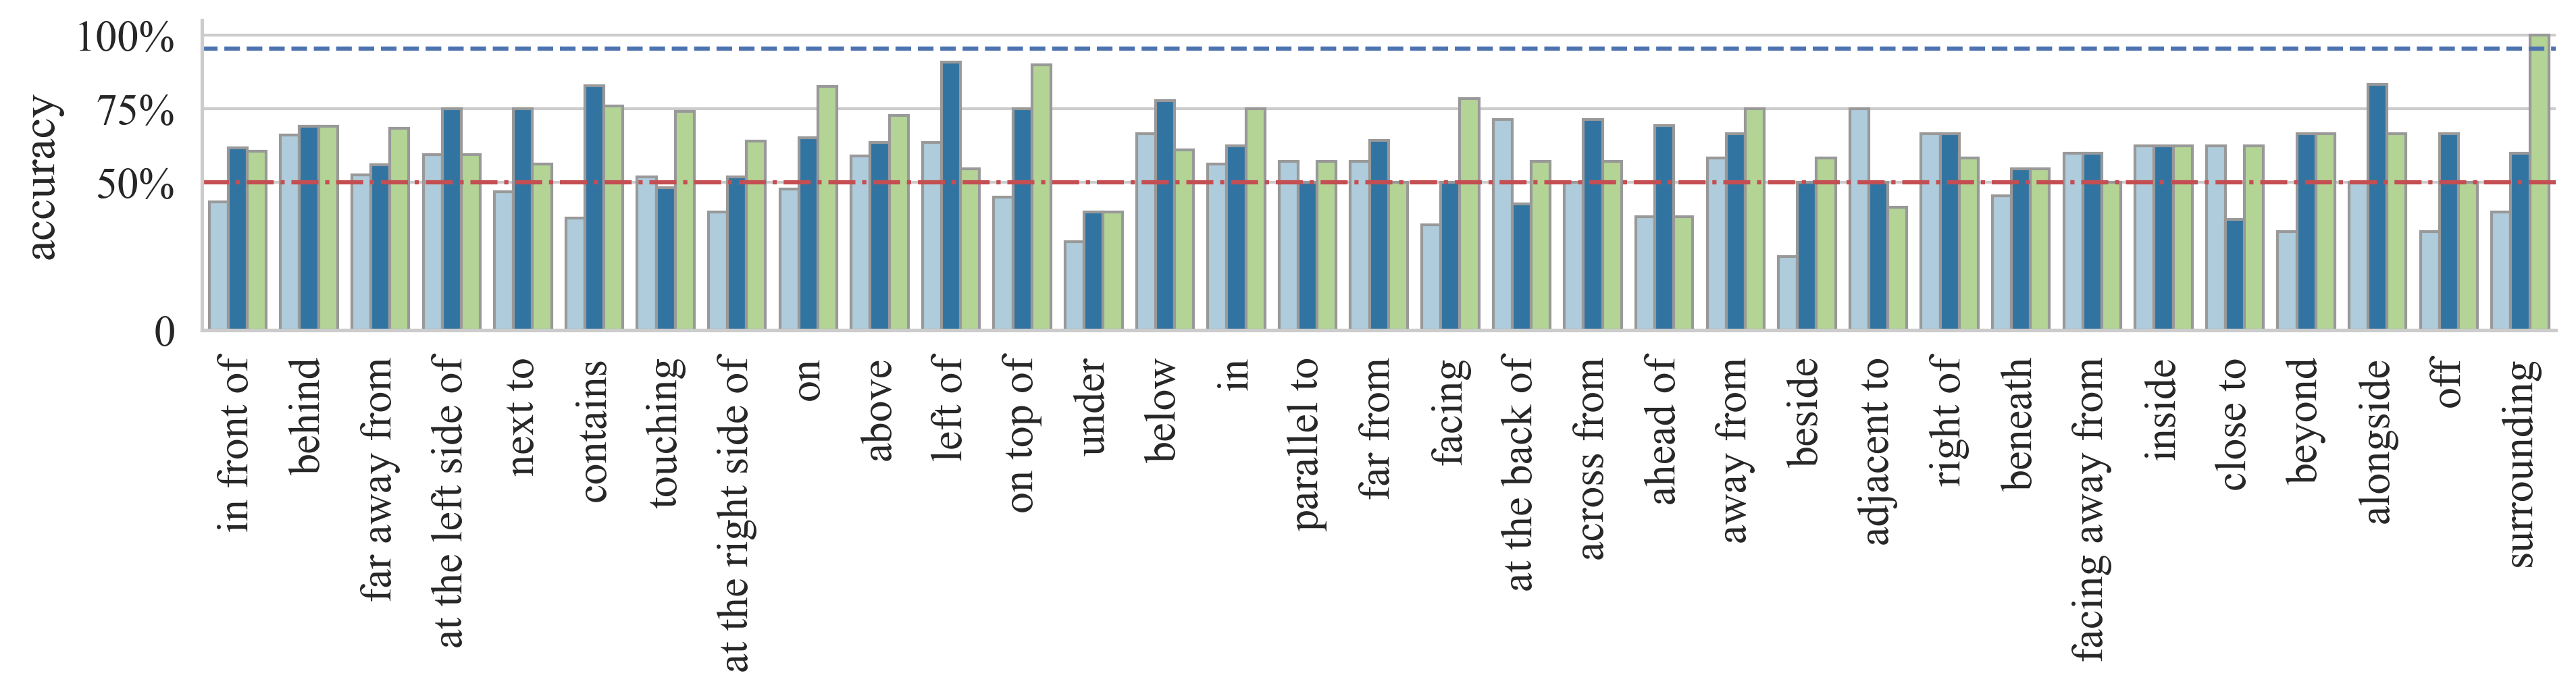
\includegraphics[width=\linewidth]{images/visual-spatial-reasoning/performance_by_relation_zeroshot_split_v2.png}
    \vspace{-1cm}
    \caption{zero-shot split}
\end{subfigure}
\caption{Performance by relation on the random (upper) and zero-shot (lower) split test sets. Relation order sorted by frequency (high to low from left to right). Only relations with more than 15 and 5 occurrences on the random and zero-shot tests respectively are shown. }
    \label{fig:performance_by_rel_base}
\end{figure*}

\subsubsection{Ours}

See \cref{fig:performance_by_rel}

\begin{figure}[ht]
    \centering
\begin{subfigure}[b]{\linewidth}
    \centering
    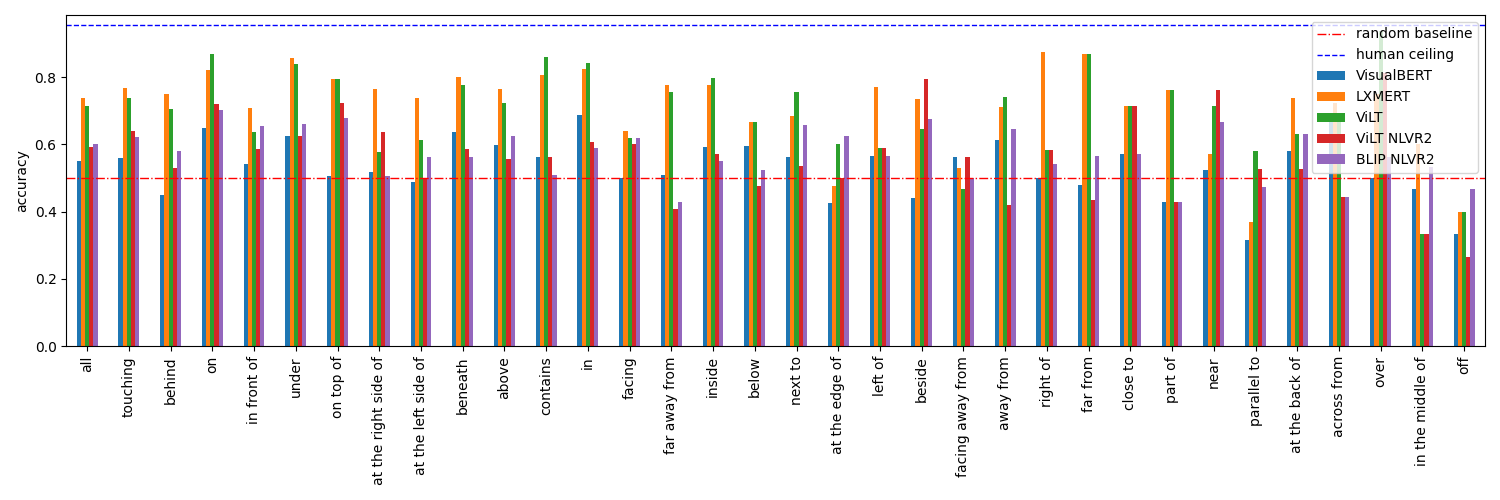
\includegraphics[width=\linewidth]{images/visual-spatial-reasoning/performance_rel_random.png}
    \vspace{-1cm}
    \caption{random split}
\end{subfigure}
\begin{subfigure}[b]{\linewidth}
    \centering
    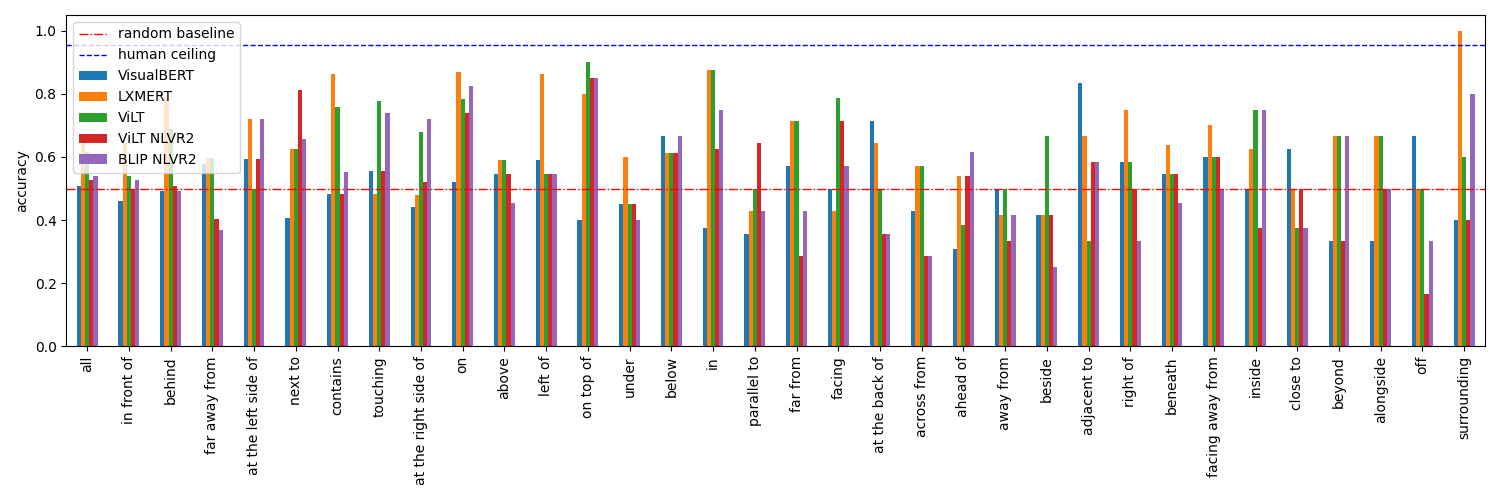
\includegraphics[width=\linewidth]{images/visual-spatial-reasoning/performance_rel_zeroshot.png}
    \vspace{-1cm}
    \caption{zero-shot split}
\end{subfigure}
\caption{Performance by relation on the random (upper) and zero-shot (lower) split test sets. Relation order sorted by frequency (high to low from left to right). Only relations with more than 15 and 5 occurrences on the random and zero-shot tests respectively are shown. }
    \label{fig:performance_by_rel}
\end{figure}

See \cref{tab:results-by-relation-random} and \cref{tab:results-by-relation-zeroshot}

\begin{table}[ht]
\centering
\begin{tabular}{lrrrrrr}
\toprule
relation &  number &  VisualBERT &  LXMERT &  ViLT &  ViLT NLVR2 &  BLIP NLVR2 \\
\midrule
all                  &    2024 &        0.55 &    0.74 &  0.71 &        0.59
&        0.60 \\
\midrule
touching             &     236 &        0.56 &    0.77 &  0.74 &        0.64 &        0.62 \\
behind               &     136 &        0.45 &    0.75 &  0.71 &        0.53 &        0.58 \\
on                   &     128 &        0.65 &    0.82 &  0.87 &        0.72 &        0.70 \\
in front of          &     116 &        0.54 &    0.71 &  0.64 &        0.59 &        0.66 \\
under                &     112 &        0.62 &    0.86 &  0.84 &        0.62 &        0.66 \\
on top of            &      87 &        0.51 &    0.79 &  0.79 &        0.72 &        0.68 \\
at the right side of &      85 &        0.52 &    0.76 &  0.58 &        0.64 &        0.51 \\
at the left side of  &      80 &        0.49 &    0.74 &  0.61 &        0.50 &        0.56 \\
beneath              &      80 &        0.64 &    0.80 &  0.78 &        0.59 &        0.56 \\
above                &      72 &        0.60 &    0.76 &  0.72 &        0.56 &        0.62 \\
contains             &      57 &        0.56 &    0.81 &  0.86 &        0.56 &        0.51 \\
in                   &      51 &        0.69 &    0.82 &  0.84 &        0.61 &        0.59 \\
facing               &      50 &        0.50 &    0.64 &  0.62 &        0.60 &        0.62 \\
far away from        &      49 &        0.51 &    0.78 &  0.76 &        0.41 &        0.43 \\
inside               &      49 &        0.59 &    0.78 &  0.80 &        0.57 &        0.55 \\
below                &      42 &        0.60 &    0.67 &  0.67 &        0.48 &        0.52 \\
next to              &      41 &        0.56 &    0.68 &  0.76 &        0.54 &        0.66 \\
at the edge of       &      40 &        0.42 &    0.48 &  0.60 &        0.50 &        0.62 \\
left of              &      39 &        0.56 &    0.77 &  0.59 &        0.59 &        0.56 \\
beside               &      34 &        0.44 &    0.74 &  0.65 &        0.79 &        0.68 \\
facing away from     &      32 &        0.56 &    0.53 &  0.47 &        0.56 &        0.50 \\
away from            &      31 &        0.61 &    0.71 &  0.74 &        0.42 &        0.65 \\
right of             &      24 &        0.50 &    0.88 &  0.58 &        0.58 &        0.54 \\
far from             &      23 &        0.48 &    0.87 &  0.87 &        0.43 &        0.57 \\
close to             &      21 &        0.57 &    0.71 &  0.71 &        0.71 &        0.57 \\
part of              &      21 &        0.43 &    0.76 &  0.76 &        0.43 &        0.43 \\
near                 &      21 &        0.52 &    0.57 &  0.71 &        0.76 &        0.67 \\
parallel to          &      19 &        0.32 &    0.37 &  0.58 &        0.53 &        0.47 \\
at the back of       &      19 &        0.58 &    0.74 &  0.63 &        0.53 &        0.63 \\
across from          &      18 &        0.67 &    0.72 &  0.67 &        0.44 &        0.44 \\
over                 &      16 &        0.50 &    0.75 &  0.94 &        0.81 &        0.56 \\
in the middle of     &      15 &        0.47 &    0.60 &  0.33 &        0.33 &        0.53 \\
off                  &      15 &        0.33 &    0.40 &  0.40 &        0.27 &        0.47 \\
\bottomrule
\end{tabular}
\caption{Number and performance by relation on the random split test. Only relations with more than 15 occurrences are shown.}
\label{tab:results-by-relation-random}
\end{table}

\begin{table}[ht]
\centering
\begin{tabular}{lrrrrrr}
\toprule
relation &  number &  VisualBERT &  LXMERT &  ViLT &  ViLT NLVR2 &  BLIP NLVR2 \\
\midrule
all                  &     731 &        0.51 &    0.66 &  0.62 &        0.53 &        0.54 \\
\midrule
in front of          &      76 &        0.46 &    0.64 &  0.54 &        0.50 &        0.53 \\
behind               &      71 &        0.49 &    0.79 &  0.69 &        0.51 &        0.49 \\
far away from        &      57 &        0.58 &    0.60 &  0.60 &        0.40 &        0.37 \\
at the left side of  &      32 &        0.59 &    0.72 &  0.50 &        0.59 &        0.72 \\
next to              &      32 &        0.41 &    0.62 &  0.62 &        0.81 &        0.66 \\
contains             &      29 &        0.48 &    0.86 &  0.76 &        0.48 &        0.55 \\
touching             &      27 &        0.56 &    0.48 &  0.78 &        0.56 &        0.74 \\
at the right side of &      25 &        0.44 &    0.48 &  0.68 &        0.52 &        0.72 \\
on                   &      23 &        0.52 &    0.87 &  0.78 &        0.74 &        0.83 \\
above                &      22 &        0.55 &    0.59 &  0.59 &        0.55 &        0.45 \\
left of              &      22 &        0.59 &    0.86 &  0.55 &        0.55 &        0.55 \\
on top of            &      20 &        0.40 &    0.80 &  0.90 &        0.85 &        0.85 \\
under                &      20 &        0.45 &    0.60 &  0.45 &        0.45 &        0.40 \\
below                &      18 &        0.67 &    0.61 &  0.61 &        0.61 &        0.67 \\
in                   &      16 &        0.38 &    0.88 &  0.88 &        0.62 &        0.75 \\
parallel to          &      14 &        0.36 &    0.43 &  0.50 &        0.64 &        0.43 \\
far from             &      14 &        0.57 &    0.71 &  0.71 &        0.29 &        0.43 \\
facing               &      14 &        0.50 &    0.43 &  0.79 &        0.71 &        0.57 \\
at the back of       &      14 &        0.71 &    0.64 &  0.50 &        0.36 &        0.36 \\
across from          &      14 &        0.43 &    0.57 &  0.57 &        0.29 &        0.29 \\
ahead of             &      13 &        0.31 &    0.54 &  0.38 &        0.54 &        0.62 \\
away from            &      12 &        0.50 &    0.42 &  0.50 &        0.33 &        0.42 \\
beside               &      12 &        0.42 &    0.42 &  0.67 &        0.42 &        0.25 \\
adjacent to          &      12 &        0.83 &    0.67 &  0.33 &        0.58 &        0.58 \\
right of             &      12 &        0.58 &    0.75 &  0.58 &        0.50 &        0.33 \\
beneath              &      11 &        0.55 &    0.64 &  0.55 &        0.55 &        0.45 \\
facing away from     &      10 &        0.60 &    0.70 &  0.60 &        0.60 &        0.50 \\
inside               &       8 &        0.50 &    0.62 &  0.75 &        0.38 &        0.75 \\
close to             &       8 &        0.62 &    0.50 &  0.38 &        0.50 &        0.38 \\
beyond               &       6 &        0.33 &    0.67 &  0.67 &        0.33 &        0.67 \\
alongside            &       6 &        0.33 &    0.67 &  0.67 &        0.50 &        0.50 \\
off                  &       6 &        0.67 &    0.50 &  0.50 &        0.17 &        0.33 \\
surrounding          &       5 &        0.40 &    1.00 &  0.60 &        0.40 &        0.80 \\
\bottomrule
\end{tabular}
\caption{Number and performance by relation on the zero-shot split test. Only relations with more than 5 occurrences are shown.}
\label{tab:results-by-relation-zeroshot}
\end{table}

\subsection{Results By Relation Meta Category}

\subsubsection{Baseline}

See \cref{fig:performance_by_meta_cat_base}

\begin{figure*}
    \centering
\begin{subfigure}[b]{0.49\linewidth}
    \centering
    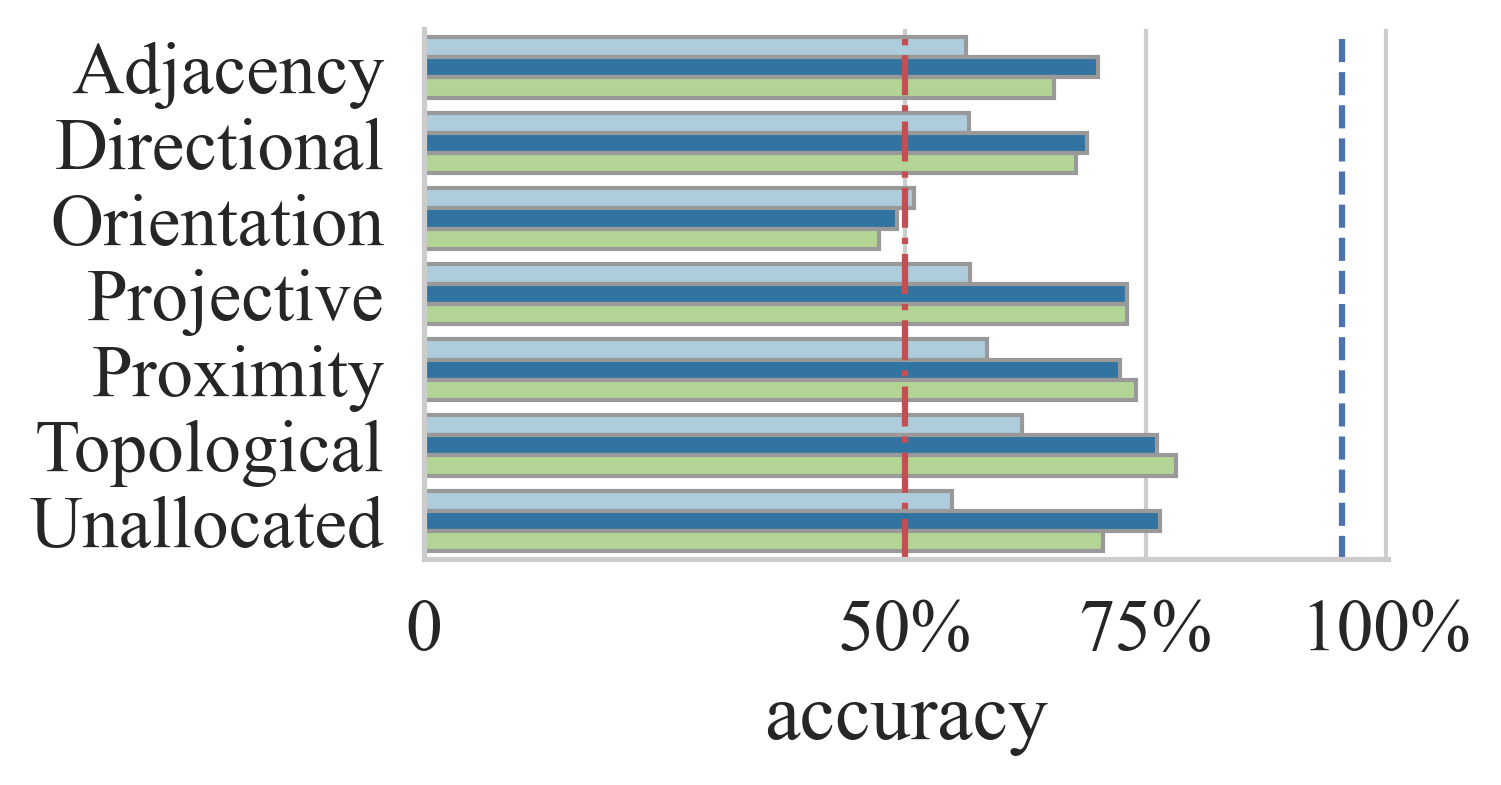
\includegraphics[width=\linewidth]{images/visual-spatial-reasoning/performance_by_meta_cat_random_split_v2.png}
    \caption{random split}
\end{subfigure}
\begin{subfigure}[b]{0.49\linewidth}
    \centering
    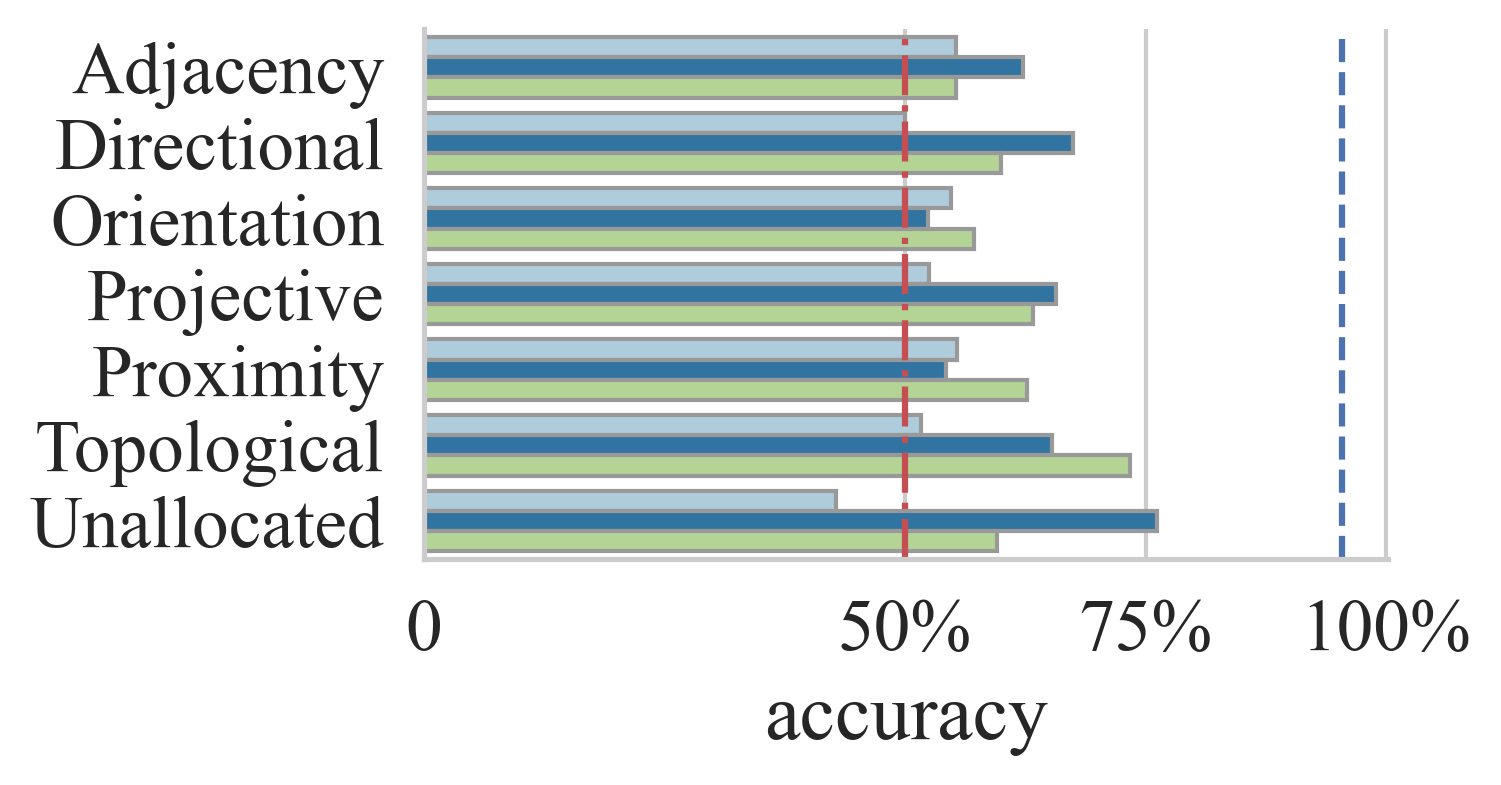
\includegraphics[width=\linewidth]{images/visual-spatial-reasoning/performance_by_meta_cat_zeroshot_split_v2.png}
    \caption{zero-shot split}
\end{subfigure}
\caption{Performance by meta categories of relations, on the random (left) and zero-shot (right) split test sets. For legend information, see \Cref{fig:performance_by_rel_base}.}
    \label{fig:performance_by_meta_cat_base}
\end{figure*}

\subsubsection{Ours}

See \cref{fig:performance_by_meta_cat}

\begin{figure}[ht]
    \centering
    \begin{subfigure}[b]{0.49\linewidth}
    \centering
    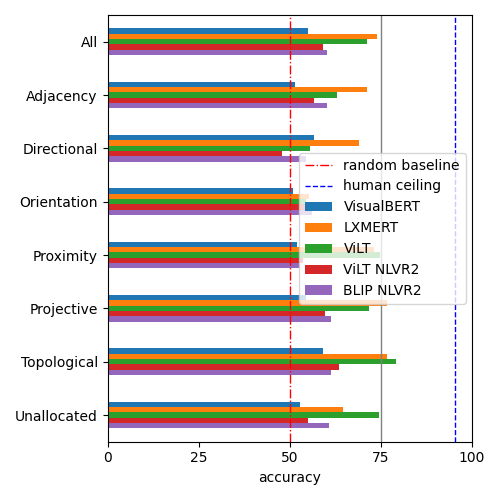
\includegraphics[width=\linewidth]{images/visual-spatial-reasoning/performance_rel_meta_cat_random.png}
    \caption{random split}
     \end{subfigure}
     \begin{subfigure}[b]{0.49\linewidth}
         \centering
    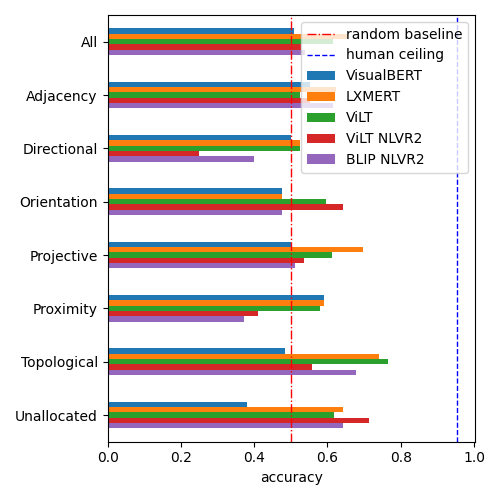
\includegraphics[width=\linewidth]{images/visual-spatial-reasoning/performance_rel_meta_cat_zeroshot.png}
         \caption{zero-shot split}
     \end{subfigure}
\caption{Performance by meta categories of relations, on the random (left) and zero-shot (right) split test sets. For legend information, see \cref{fig:performance_by_rel}.}
    \label{fig:performance_by_meta_cat}
\end{figure}

See \cref{tab:results-by-relation-meta-category-random} and \cref{tab:results-by-relation-meta-category-zeroshot}

\begin{table}[ht]
\centering
\begin{tabular}{lrrrrrr}
\toprule
category &  number &  VisualBERT &  LXMERT &  ViLT &  ViLT NLVR2 &  BLIP NLVR2 \\
\midrule
All         &    2024 &        0.55 &    0.74 &  0.71 &        0.59 &        0.60 \\
\midrule
Adjacency   &     284 &        0.51 &    0.71 &  0.63 &        0.57 &        0.60 \\
Directional &      90 &        0.57 &    0.69 &  0.56 &        0.48 &        0.54 \\
Orientation &     112 &        0.51 &    0.55 &  0.54 &        0.55 &        0.56 \\
Projective  &     773 &        0.54 &    0.77 &  0.72 &        0.60 &        0.61 \\
Proximity   &     123 &        0.52 &    0.73 &  0.75 &        0.54 &        0.53 \\
Topological &     591 &        0.59 &    0.77 &  0.79 &        0.63 &        0.61 \\
Unallocated &      51 &        0.53 &    0.65 &  0.75 &        0.55 &        0.61 \\
\bottomrule
\end{tabular}
\caption{Number and performance by relation meta category on the random split test.}
\label{tab:results-by-relation-meta-category-random}
\end{table}

\begin{table}[ht]
\centering
\begin{tabular}{lrrrrrr}
\toprule
category &  number &  VisualBERT &  LXMERT &  ViLT &  ViLT NLVR2 &  BLIP NLVR2 \\
\midrule
All         &     731 &        0.51 &    0.66 &  0.62 &        0.53 &        0.54 \\
\midrule
Adjacency   &     114 &        0.55 &    0.62 &  0.53 &        0.55 &        0.61 \\
Directional &      40 &        0.50 &    0.52 &  0.52 &        0.25 &        0.40 \\
Orientation &      42 &        0.48 &    0.48 &  0.60 &        0.64 &        0.48 \\
Projective  &     286 &        0.50 &    0.70 &  0.61 &        0.54 &        0.51 \\
Proximity   &      83 &        0.59 &    0.59 &  0.58 &        0.41 &        0.37 \\
Topological &     124 &        0.48 &    0.74 &  0.77 &        0.56 &        0.68 \\
Unallocated &      42 &        0.38 &    0.64 &  0.62 &        0.71 &        0.64 \\
\bottomrule
\end{tabular}
\caption{Number and performance by relation meta category on the zero-shot split test.}
\label{tab:results-by-relation-meta-category-zeroshot}
\end{table}
